\section{Method}
\label{sec:method}

The method has three moving parts and they can be read in order. First, the LLM's own surprise picks out candidate event boundaries (\cref{sec:method-segmentation}). Second, a graph-theoretic refinement step nudges those boundaries to positions that group similar keys together (\cref{sec:method-refinement}). Third, the events stored under the resulting segmentation are pulled back into the LLM's context through two complementary buffers (\cref{sec:method-retrieval}). Everything runs at inference time on a frozen base model.

\subsection{Event segmentation via Bayesian surprise}
\label{sec:method-segmentation}

The segmentation step asks a simple question of every token: did the model find this token unexpected? If yes, the token is a candidate event boundary. If no, the token continues the current event. The boundary detector is built on quantities the model already produces.

\paragraph{Surprise.}
For an autoregressive LLM with parameters $\theta$, the conditional probability $P(x_t \mid x_{<t}; \theta)$ is computed during the normal forward pass. The Bayesian surprise of the actually observed token $x_t$ is
\begin{equation}
  \Surprise(x_t) \;=\; -\log P(x_t \mid x_{<t}; \theta).
  \label{eq:surprise}
\end{equation}
This is the same quantity the cross-entropy loss is built on; the only twist is that EM-LLM uses it as a runtime feature rather than as a training signal.

\paragraph{Threshold rule.}
A token at position $t$ is treated as a candidate boundary when its surprise exceeds a moving threshold
\begin{equation}
  T_t \;=\; \mu_{t-\tau:t} \;+\; \gamma \, \sigma_{t-\tau:t},
  \label{eq:threshold}
\end{equation}
where $\mu_{t-\tau:t}$ and $\sigma_{t-\tau:t}$ are the running mean and standard deviation of $\Surprise$ over the trailing window of length $\tau$, and $\gamma$ is a fixed scaling constant. \cref{eq:threshold} is Eq.\ 1 of the paper. Two design choices are worth pulling out. First, $T_t$ adapts to the local distribution, which means a stretch of unusually predictable text (the middle of a procedural document, say) does not get over-segmented just because its absolute surprise is low. Second, $\gamma$ is the only knob a user typically tunes; the paper sweeps $\gamma \in \{1.0, 1.5, 2.0, 2.5, 3.0, 3.5\}$ and reports $\gamma = 1.0$ as the best default across all tested base models.

\paragraph{Worked example.}
Suppose the trailing window has mean surprise $\mu = 2.0$ and standard deviation $\sigma = 0.5$, and we use $\gamma = 1.0$. Then the threshold for the next token is $T = 2.0 + 1.0 \cdot 0.5 = 2.5$. Now imagine six consecutive surprises:
\begin{center}
\begin{tabular}{lcccccc}
  \toprule
  token index $t$    & 1   & 2   & 3   & 4   & 5   & 6 \\
  $\Surprise(x_t)$   & 1.9 & 2.4 & 3.1 & 2.0 & 1.8 & 2.7 \\
  boundary?          & no  & no  & yes & no  & no  & yes \\
  \bottomrule
\end{tabular}
\end{center}
Tokens 3 and 6 trip the threshold and enter the candidate boundary list $B$. Their surprise values are not the largest possible; what matters is that they exceed the local mean by more than $\gamma$ standard deviations. In a real run, $\mu$ and $\sigma$ themselves are updated as the window slides forward, so the threshold at token 6 reflects a different local distribution than the threshold at token 3.

\paragraph{Outputs of this step.}
After segmentation the system holds a list $B = (b_1, b_2, \dots, b_k)$ of candidate boundary positions. Each $b_i$ is a token index where $\Surprise$ exceeded the threshold. The interval $[b_i, b_{i+1})$ is a proposed event. These intervals are still provisional; the refinement step below moves the right edge of each interval to a nearby position that produces a more coherent group of keys.

\subsection{Boundary refinement via graph clustering}
\label{sec:method-refinement}

Surprise tells us \emph{where} the model was caught off guard. It does not, by itself, tell us where the cleanest split between two events lies. A high-surprise token might land a few positions before the actual semantic break, or a few positions after it. The refinement step closes that gap by looking at the similarity structure of the attention keys.

\paragraph{Similarity graph.}
For attention head $h$, the key vectors $K^h_1, \dots, K^h_n$ over the current local window can be assembled into a similarity matrix
\begin{equation}
  A^h_{ij} \;=\; \mathrm{sim}(K^h_i, K^h_j) \;=\; (K^h_i)^\top K^h_j,
  \label{eq:adjacency}
\end{equation}
which is Eq.\ 2 of the paper. The choice of dot product (rather than cosine or another distance) is deliberate: the same similarity drives the LLM's own attention scores, so optimising group structure under $A^h$ is more aligned with the model's downstream computation than optimising under a generic distance would be. Reading $A^h$ as the weighted adjacency matrix of a graph over tokens, the question becomes which partition of those tokens into contiguous segments forms the best community structure.

\paragraph{Modularity.}
Modularity is the network-science measure of how much more strongly connected nodes within a community are than would be expected by chance. For a partition with community labels $c_i$ and total edge weight $m = \sum_{ij} A^h_{ij}/2$,
\begin{equation}
  \Modularity(A^h, B) \;=\; \frac{1}{4m} \sum_{i,j} \left( A^h_{ij} - \frac{1}{2m} \sum_i A^h_{ij} \sum_j A^h_{ij} \right) \delta(c_i, c_j),
  \label{eq:modularity}
\end{equation}
where $\delta$ is the Kronecker delta (Eq.\ 3 of the paper). Higher modularity means edges concentrate inside communities. The refinement step seeks boundaries that maximise $\Modularity$.

\paragraph{Conductance.}
Conductance is the complementary measure. It looks at the fraction of total edge weight cut at a community boundary. For a candidate community $S \subset V$,
\begin{equation}
  \Conductance(A^h, B) \;=\; \min_{S \in V} \frac{\sum_{i \in S, j \notin S} A^h_{ij}}{\min(\mathrm{vol}(S), \mathrm{vol}(V \setminus S))},
  \label{eq:conductance}
\end{equation}
with $\mathrm{vol}(S) = \sum_{i,j \in S} A_{ij}$ (Eq.\ 4 of the paper). Lower conductance means the cut at the boundary is small relative to the internal density of either side. Refinement under conductance picks boundaries that minimise $\Conductance$.

\paragraph{The refinement algorithm.}
With either metric in hand, the algorithm walks the candidate boundary list and adjusts each boundary to the position that optimises the chosen score on the induced subgraph. Pseudocode appears in \cref{alg:segmentation}, which follows Algorithm 1 of the paper.

\begin{algorithm}[h]
  \DontPrintSemicolon
  \KwIn{Token sequence \texttt{tok}, threshold $T$, metric function $f$}
  \KwOut{Final boundary positions $B$}
  $B \gets \{\, i \in \{1, \dots, |\texttt{tok}|\} \mid -\log P(\texttt{tok}[i]) > T \,\}$ \tcp*[r]{surprise boundaries}
  \For{$i \gets 1$ \KwTo $|B| - 1$}{
    $\alpha, \beta \gets B[i],\ B[i+1]$\;
    $B[i+1] \gets \arg\max_{\hat{\beta} \in (\alpha, \beta]} f\big(A,\ \{\alpha, \hat{\beta}\}\big)$ \tcp*[r]{shift boundary}
  }
  \Return $B$\;
  \caption{Event segmentation in the KV cache, following Algorithm 1 of \textcite{fountas2025emllm}.}
  \label{alg:segmentation}
\end{algorithm}

\begin{figure}[h]
\centering
% Boundary refinement viewed as a graph cut on the key similarity matrix.
% A small toy example: 8 tokens, surprise picks position 4 as a candidate
% boundary; refinement evaluates positions 3 and 5 too and picks the one
% whose induced two-community split scores best.

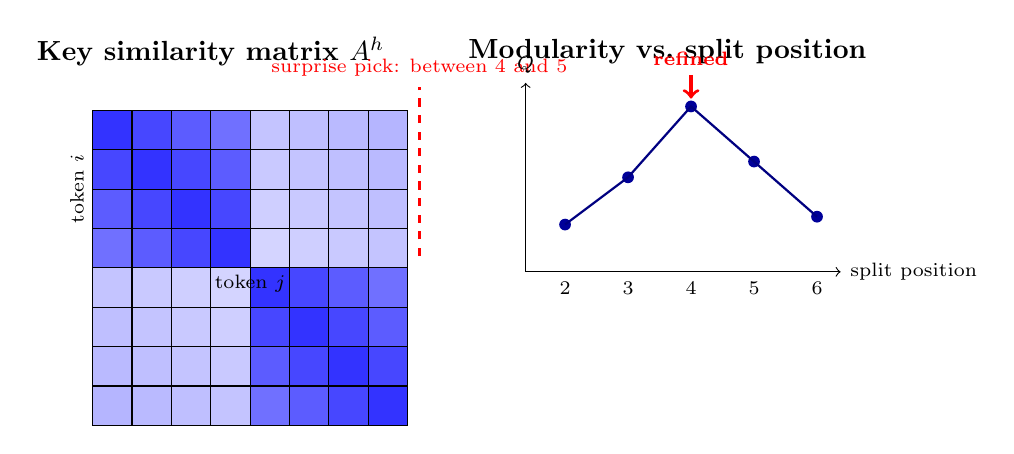
\begin{tikzpicture}[
  font=\footnotesize,
  cell/.style={draw, rectangle, minimum width=0.5cm, minimum height=0.5cm, inner sep=0pt},
  node distance=0.5cm,
]

% --- Left panel: similarity matrix as a heatmap ---
\begin{scope}[xshift=0cm, yshift=0cm]
  \node[font=\bfseries] at (2.0, 3.0) {Key similarity matrix $A^h$};

  % Generate an 8x8 grid with two block-diagonal communities at positions 1-3 and 5-8.
  % Color intensity ~ similarity. Within-cluster is darker.
  \foreach \i in {1,...,8} {
    \foreach \j in {1,...,8} {
      \pgfmathsetmacro{\val}{
        ifthenelse((\i<5 && \j<5) || (\i>4 && \j>4),
          80 - 8*abs(\i-\j),    % within-cluster
          15 + 2*abs(\i-\j))    % across-cluster
      }
      \pgfmathsetmacro{\colorval}{min(100, max(5, \val))}
      \node[cell, fill=blue!\colorval!white]
        at ({\j*0.5 + 0.25}, {2.5 - \i*0.5}) {};
    }
  }

  % Candidate boundary line at position 4-to-5 (surprise pick).
  \draw[red, very thick, dashed] (4.65, 0.4) -- (4.65, 2.55) node[above, font=\scriptsize] {surprise pick: between 4 and 5};

  % Axis labels.
  \node[font=\scriptsize] at (2.5, 0.05) {token $j$};
  \node[font=\scriptsize, rotate=90] at (0.3, 1.25) {token $i$};
\end{scope}

% --- Right panel: modularity score at each candidate split position ---
\begin{scope}[xshift=6.0cm, yshift=0.2cm]
  \node[font=\bfseries] at (1.8, 2.8) {Modularity vs.\ split position};

  % Axes
  \draw[->] (0, 0) -- (4.0, 0) node[right, font=\scriptsize] {split position};
  \draw[->] (0, 0) -- (0, 2.4) node[above, font=\scriptsize] {$Q$};

  % Data points: a peak at position 4 (correct boundary), lower at 3 and 5.
  \foreach \x/\y/\lbl in {0.5/0.6/2, 1.3/1.2/3, 2.1/2.1/4, 2.9/1.4/5, 3.7/0.7/6} {
    \node[circle, fill=blue!60!black, inner sep=1.5pt] at (\x, \y) {};
    \node[below, font=\scriptsize] at (\x, 0) {\lbl};
  }

  % Connect them.
  \draw[blue!50!black, thick]
    (0.5, 0.6) -- (1.3, 1.2) -- (2.1, 2.1) -- (2.9, 1.4) -- (3.7, 0.7);

  % Mark the chosen split with a red arrow.
  \draw[red, very thick, ->] (2.1, 2.5) -- (2.1, 2.2);
  \node[red, font=\scriptsize\bfseries, above] at (2.1, 2.5) {refined};
\end{scope}

\end{tikzpicture}

\caption{Refinement as a graph cut. Left: the key similarity matrix has two soft communities (positions 1--4 and 5--8) with a band of weak cross-cluster similarity in between. The surprise threshold marks position 4--5 as a candidate boundary. Right: modularity is evaluated at each candidate split position within a refinement window; the position that maximises $Q$ is the refined boundary.}
\label{fig:boundary-refinement}
\end{figure}

\paragraph{Why it helps and what it costs.}
The intuition is that surprise picks out the rough location of an event change but the precise location can sit one or two tokens to either side of the surprise spike. The refinement step lets the similarity structure of the keys speak. If $\alpha$ and $\beta$ are adjacent candidate boundaries, the algorithm searches positions strictly between them and picks the one whose induced split scores best under $f$. The complexity is $O(nm)$ where $n$ is the sequence length and $m$ is the chunk size used to process the sequence (Appendix C.1 of the paper); in practice $m$ is set so that the refinement cost is small compared with the cost of the attention itself. The paper reports modularity slightly outperforming conductance on the experimental tasks, but both improve over surprise alone.

\subsection{Two-stage memory retrieval}
\label{sec:method-retrieval}

Once events are stored, the question is which ones to bring back when the LLM generates the next token. EM-LLM's answer combines two retrieval signals, one based on content similarity and one based on temporal neighbourhood. Each transformer layer runs both independently.

\paragraph{Stage one: similarity buffer.}
For the current attention query, the system performs a $k$-nearest-neighbour lookup over stored events. The key used for the comparison is not the full event but a small set of \emph{representative tokens} per event, chosen as the most influential tokens within the event in the sense of \textcite{xiao2024infllm}. The top $k_s$ events by dot-product similarity to the query enter the similarity buffer. For small memories this lookup is exact; for memories large enough to spill to CPU or disk (the 10M-token regime in particular) the implementation uses an approximate $k$-NN library.

\paragraph{Stage two: contiguity buffer.}
When an event is retrieved by similarity, EM-LLM also enqueues its temporal neighbours, the events that originally fell within $\pm n$ positions in the source sequence (the paper uses $n = 1$ throughout). The contiguity buffer is a fixed-size queue of capacity $k_c$. When the queue fills, older or already-attended events are dequeued. This is the operational analogue of the contiguity effect from \cref{sec:episodic}: items studied close together in time should be available together at recall.

\begin{figure}[h]
\centering
% Two-stage retrieval. Each transformer layer runs both stages independently.
% Used in Chapter 3 (method) and referenced from Chapter 8 (walkthrough).

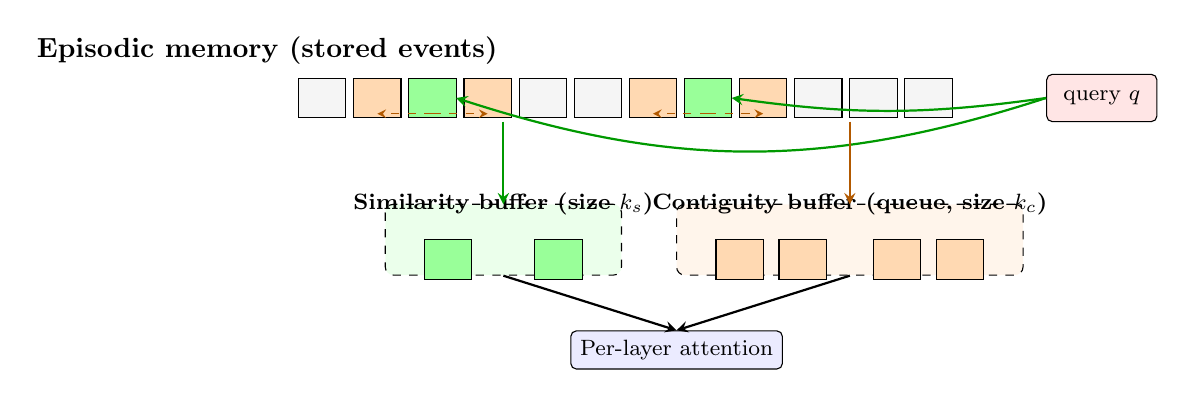
\begin{tikzpicture}[
  font=\footnotesize,
  event/.style={draw, rectangle, minimum width=0.6cm, minimum height=0.5cm, inner sep=1pt},
  query/.style={draw, rounded corners=2pt, fill=red!10, minimum width=1.4cm, minimum height=0.6cm},
  buffer/.style={draw, dashed, rounded corners=3pt, inner sep=6pt},
  arrow/.style={->, >=stealth, thick},
  faded/.style={fill=gray!8},
]

% Event store: a row of 12 stored events with two highlighted as top-k hits.
\node[font=\bfseries] at (0, 1.8) {Episodic memory (stored events)};
\foreach \i in {1,...,12} {
  \node[event, faded] (e\i) at (\i * 0.7, 1.2) {};
}
% Two top-similarity hits, dark green.
\node[event, fill=green!40] at (3 * 0.7, 1.2) {};
\node[event, fill=green!40] at (8 * 0.7, 1.2) {};
% Neighbours of the hits (enqueued into contiguity buffer), light orange.
\node[event, fill=orange!30] at (2 * 0.7, 1.2) {};
\node[event, fill=orange!30] at (4 * 0.7, 1.2) {};
\node[event, fill=orange!30] at (7 * 0.7, 1.2) {};
\node[event, fill=orange!30] at (9 * 0.7, 1.2) {};

% Query at the right.
\node[query] (q) at (10.6, 1.2) {query $q$};

% Similarity arrows (curved, green).
\draw[arrow, green!60!black] (q.west) to[bend left=18] (3 * 0.7 + 0.3, 1.2);
\draw[arrow, green!60!black] (q.west) to[bend left=8]  (8 * 0.7 + 0.3, 1.2);

% Contiguity arrows (curved, orange) from green hits to their neighbours.
\draw[->, >=stealth, dashed, orange!70!black] (3 * 0.7, 1.0) -- (2 * 0.7, 1.0);
\draw[->, >=stealth, dashed, orange!70!black] (3 * 0.7, 1.0) -- (4 * 0.7, 1.0);
\draw[->, >=stealth, dashed, orange!70!black] (8 * 0.7, 1.0) -- (7 * 0.7, 1.0);
\draw[->, >=stealth, dashed, orange!70!black] (8 * 0.7, 1.0) -- (9 * 0.7, 1.0);

% The two buffers below.
\node[buffer, fill=green!8, minimum width=3.0cm, minimum height=0.9cm] (simbuf) at (3.0, -0.6) {};
\node[font=\footnotesize\bfseries] at (3.0, -0.15) {Similarity buffer (size $k_s$)};
\node[event, fill=green!40] at (2.3, -0.85) {};
\node[event, fill=green!40] at (3.7, -0.85) {};

\node[buffer, fill=orange!8, minimum width=4.4cm, minimum height=0.9cm] (cbuf) at (7.4, -0.6) {};
\node[font=\footnotesize\bfseries] at (7.4, -0.15) {Contiguity buffer (queue, size $k_c$)};
\node[event, fill=orange!30] at (6.0, -0.85) {};
\node[event, fill=orange!30] at (6.8, -0.85) {};
\node[event, fill=orange!30] at (8.0, -0.85) {};
\node[event, fill=orange!30] at (8.8, -0.85) {};

% Arrows from the event store into the two buffers.
\draw[arrow, green!60!black] (3.0, 0.9) -- (3.0, -0.15);
\draw[arrow, orange!70!black] (7.4, 0.9) -- (7.4, -0.15);

% Final union arrow into attention.
\node[font=\footnotesize, draw, rounded corners=2pt, fill=blue!8, minimum width=2.4cm] (attn) at (5.2, -2.0) {Per-layer attention};
\draw[arrow] (simbuf.south) -- (attn.north);
\draw[arrow] (cbuf.south) -- (attn.north);

\end{tikzpicture}

\caption{Two-stage retrieval for one generation step. The similarity buffer picks the $k_s$ events whose representative tokens best match the current query under dot-product similarity (solid green arrows). The contiguity buffer enqueues the temporal neighbours of those events (dashed orange arrows). Both feed into the per-layer attention.}
\label{fig:two-stage-retrieval}
\end{figure}

\paragraph{Total context.}
The total number of retrieved events at each step is $k = k_s + k_c$. The paper expresses experimental settings in tokens rather than events, so configurations like ``4k local + 4k retrieved'' refer to maximum token budgets. The split between similarity and contiguity is controlled by the contiguity ratio $k_r = k_c / k$. The paper sweeps $k_r \in \{0.3, 0.5, 0.7\}$ and reports $k_r = 0.3$ as a robust default; the similarity buffer dominates by token count, with the contiguity buffer playing a smaller, supplementary role.

\paragraph{Per-layer independence.}
Every transformer layer carries out its own retrieval. This is one of the design choices that most clearly separates EM-LLM from prompt-level RAG. A RAG system attends to retrieved chunks once, at the input layer, and then every later layer reads transformed versions of the same retrieved content. EM-LLM lets different layers pull in different events from the same memory store. The paper argues (Section~4.1, Fig.~1) that this per-layer flexibility is the main source of its 30.5-point LongBench advantage over the NV-Embed-v2 RAG baseline.

\paragraph{Putting the pieces together.}
For each generated token, each layer attends to four regions in sequence: the 128 initial-token attention sinks, the contiguity buffer (events temporally adjacent to recently retrieved events), the similarity buffer (events most similar to the current query), and the local context window of recent tokens (working memory). Tokens outside these regions are invisible to the softmax at that step. Memory beyond the local window is not lost; it is just not loaded into attention until similarity or contiguity calls for it. \cref{sec:architecture} formalises this layout and walks through how RoPE and the patch into Hugging Face transformers actually carry it out at the code level.
